%%%%%%%%%%%%%%%%%%%%%%%%%%%%%%%%%%%%%%%%%%%%%%%%%%%%%%%%%%%%%%%%%%%%%%%%%%%%
%% Thesis Template - Tilburg Science Hub
%% Andrea Domenico Antonacci, a.d.antonacci@tilburguniversity.edu
%% Last update: April 2021
%% Use pdflatex
%%%%%%%%%%%%%%%%%%%%%%%%%%%%%%%%%%%%%%%%%%%%%%%%%%%%%%%%%%%%%%%%%%%%%%%%%%%%

%% INSTRUCTIONS:
%% Use this file to define the document structure, the preamble, the abstract, and the acknowledgements.
%% Use the section files to write your content and import them here.
%% This template is meant to run on pdflatex and with fonts available via packages.
%% Use XeLaTeX if you want to use your own custom fonts.

\RequirePackage{amsmath} % Load amsmath first
\documentclass[a4paper,12pt]{article}
% Set your margins here
\usepackage[margin=1in]{geometry}
% Set your language
\usepackage[english]{babel}
\usepackage[utf8]{inputenc}
% Define fonts via packages
\usepackage{mathpazo} % Use Palatino font
% \usepackage{gfsdidot} % Or use Didot font
% Set global line spacing
\renewcommand{\baselinestretch}{1.5}
% Allow multi-column environments
\usepackage{multicol}
\setlength\columnsep{40pt}
% Formulas and math
\usepackage{amssymb}
\usepackage{mathtools}
\usepackage{empheq}
\usepackage{units} % Allow nice in-line, diagonal fractions
% Define bibliography, update according to your needs
\usepackage[
    backend=biber,
    style=numeric,
  ]{biblatex}
 \addbibresource{bib.bib}
% Allow hyperref with click-through sections and references
\usepackage[unicode=true,pdfusetitle,bookmarks=true,bookmarksnumbered=true,bookmarksopen=true,bookmarksopenlevel=1,breaklinks=false,pdfborder={0 0 0},pdfborderstyle={},backref=false]{hyperref}
% Replace "Placeholder Name" in pdfauthor with your real name and update the link colors to taste
\hypersetup{pdfpagelayout=OneColumn, pdfnewwindow=true, pdfstartview=XYZ, plainpages=false,pdfauthor={Placeholder Name},colorlinks=true,linkcolor=ForestGreen,citecolor=ForestGreen}
% Allow fancy headers
\usepackage{fancyhdr}
\fancypagestyle{SectionFirstPage}{\fancyhead{}\renewcommand{\headrulewidth}{0pt}} % Use this pagestyle to hide headers on the first page of sections
% Misc packages
\usepackage{lipsum} % For prototyping
\usepackage{listings} % To highlight code
\usepackage{algorithm} % For algorithms
\usepackage{setspace} % To set line spacing locally
\usepackage{graphicx} % Allow figures
\graphicspath{ {images/} } % Specify the path for images
\usepackage[dvipsnames]{xcolor} % Enable more colors in text
\usepackage{microtype} % Improve justification
\usepackage{url} % Line-breaking urls
\usepackage{pdflscape} % Allow pages in landscape mode
\usepackage{multirow} % Allow multirow in tables
\usepackage[labelfont=bf]{caption} % Set caption distances from tables and figures
\usepackage{subcaption} % For subfigures, remove if unused
\captionsetup[table]{skip=10pt, position=top}
\captionsetup[figure]{belowskip=10pt, skip=5pt, position=top}
\usepackage[nottoc]{tocbibind} % Add bibliography to Table of Content
\usepackage{makecell} % Allow to break lines inside a table cell
\usepackage[para]{threeparttable} % For structured and complex tables
\usepackage{rotating} % To rotate tables
\usepackage{textcomp} % For symbols
\usepackage{tikz} % For graphs and graphics
\usetikzlibrary{shapes.geometric, shapes.misc, arrows, positioning}
\def\checkmark{\tikz\fill[scale=0.4](0,.35) -- (.25,0) -- (1,.7) -- (.25,.15) -- cycle;} % Define a checkmark (tick), used in section 2
\usepackage{varioref} % Intelligent references with pageref automatically added
\setlength{\headheight}{14.49998pt}
\counterwithin*{equation}{section} % Reset numbering for each chapter
\counterwithin*{equation}{subsection}
\newenvironment{system}%
{\left\lbrace\begin{array}{@{}l@{}}}%
{\end{array}\right.}
% Define title page
\usepackage{titling}
\renewcommand\maketitlehooka{\null\mbox{}\vfill} % To vertically center it
\renewcommand\maketitlehookd{\vfill\null}
\title{
    Belote AI \\
        \large Project in Artificial Intelligence and Decision Support \\ American University of Armenia \\
}
\author{Grigor Hovhannisyan
\and
Aram Abrahamyan
\and
Meruzhan Khachatryan
\and
Mikayel Davtyan
}
% \date{January 2000} % Uncomment for custom date

%%%%%%%%%%%%%%%%%%%%%%%%%%%%%%%%%%%%%%%%%%%%%%%%%%%%%%%%%%%%%%%%%%%%%%%%%%%%
%% CONTENT BELOW
%%%%%%%%%%%%%%%%%%%%%%%%%%%%%%%%%%%%%%%%%%%%%%%%%%%%%%%%%%%%%%%%%%%%%%%%%%%%

\begin{document}
\pagecolor{black}
\color{white}

% Title page
{ % Use curly brackets to create a group and assign properties locally
\setstretch{1.0}
\maketitle\thispagestyle{empty}
\vspace{1cm}{}
}
\vspace{1cm}


% Table of Content
{
    \newpage
    \pagenumbering{arabic}
    \setstretch{1.0}
    \hypersetup{linkcolor=white} % Links in TOC are black
    \tableofcontents
}

% Abstract
\newpage
\pagenumbering{roman}
\begin{abstract}
    \addcontentsline{toc}{section}{Abstract}
    The game Bazar Blot is a very popular game originating in France and making it's way into Armenia with heavy modifications.
    In this paper we will thoroughly explain the rules of the game, discuss how one might try to implement an agent for the game and show some examples of how we managed to do it.
    The game in itself is very complex involving enough rules to barely fit in 4-5 pages and requires a lot of effort to understand.
    The agents for the game available now are generally accepted to be very bad at the game, while reading the paper we hope it will be apparent why that is the case.
    In order to demonstrate the agents we also made the game using Python that entirely runs inside a terminal which is available in our GitHub page.
\end{abstract}

% Content
\newpage
\pagestyle{fancy} % Initiate headers
% Define global headers for all the sections
\lhead{\nouppercase{\rightmark}}
\rhead{}
\pagenumbering{arabic}
% Import sections
\section{Bazar Blot Game}\label{GameIntro}\thispagestyle{SectionFirstPage} % Hide headers on the first page of the section
\lhead{Introduction to Bazar Blot}
\subsection{The Origin of the Game}
\hspace{\parindent} Belote is a 32-card game played primarily in France and in some other countries like Armenia, Belgium, Bulgaria, Croatia, Cyprus, and Georgia.
In each country, the game has encountered some modifications; however, the fundamental rules are mostly identical everywhere.
Firstly, it would be more accurate to introduce the original game, Belote, and then add the Armenian modifications to get the overall understanding of Bazar Blot's rules and gameplay.
The game appeared around 1900 in France and is one of the most popular card games in France and other European countries.
The rules were first published in French in 1921.
The name of the game \textit{``Belote''} has possibly originated from the term used to describe a pair of \textit{King} and \textit{Queen} of a trump suit, which gives 2 bonus points to the pair of players when one of them has this combination.
This name also varies from region to region.
In Saudi Arabia, it is called \textit{Baloot}, in Cyprus, the name is \textit{Pilotta}, and in Armenia, it is known as \textit{Blot}.
\subsection{General Rules}
\hspace{\parindent} Belote is played with a \textit{Piquet} deck, which is a standard deck stripped from 2 to 6's, meaning it has 4 suits: \textit{Spades, Hearts, Clubs, Diamonds} and 8 ranks: \textit{A, K, Q, J, 10, 9, 8, 7}.
The game is played with 2 teams of 2 players and playing in the turn counterclockwise.
The deck is typically shuffled and offered the player preceding the dealer to cut the deck.
The cutter may cut or just tap on the top of the pack in which case no cutting is done.
The first dealing is done by the winners of the previous game, which in Armenia sometimes is called ``Pativ tal''.
The cards are dealt counterclockwise, starting from the dealer's successor.
In the original version, each player receives a pack of 3 cards, then another set of 2.
The remains faced down until the contract is being agreed.
The remaining cards are dealt after the bidding – a group of three for each player except the player who got the card that was in the middle, who gets two.
In the Armenian \textit{``Bazar Blot''} version, each player gets a pack of 4 cards, then another equal pack, after which the bidding process starts.
\subsection{Bidding}
The possible contracts for \textit{``Bazar Blot''} are:
\begin{itemize}
    \item Clubs $\clubsuit$
    \item Diamonds $\diamondsuit$
    \item Hearts $\heartsuit$
    \item Spades $\spadesuit$
    \item No Trumps
\end{itemize}
Every player must either suggest a higher bid or:
\begin{itemize}
    \item Pass
    \item Double (Coinchee or contra), if they are sure the opponents will not be able to get that many points.
    \item Re-Double (Re-contra), if the other team have doubled bidder's or bidder partner's contract.
    \item Capot, meaning that team will win the round without giving any points to the opponents.
\end{itemize}

The bidding procedure is over when one of the following happens:
\begin{itemize}
    \item Four \textit{passes} are announced.
    \item A contract is \textit{Doubled} and (and not) \textit{Re-Doubled}
\end{itemize}

\subsection{Playing}
The dealer's successor(the player to the right of the dealer) plays their card first.
The first player can play any card; however, the subsequent players must follow the suit if they can.
If they do not have a card of the same suit, they must play a trump card.
If they cannot play trump either, they can play any suit.
If the first card played is trump, the subsequent players must follow the suit as well as play a trump card that beats all the cards on the table if they can.
It is called \textit{``raising''} and applies only for trump suits.
If they cannot play such card, they put any trump card.
In case they do not have any trump, they can play any suit.
If non-trump card was played first, and then trump, the subsequent player must follow the suit of the first card, and does not have to put a higher trump; however, if the player on turn does not have a card that follows the suit of the first card, they have to put a higher trump.
If any of the above rules are being broken, the opponents get 162 points in addition to all \textit{``declarations''} declared in the round regardless of who has made the declaration and current round ends.
When each player has played 1 card, the player whose card was the highes wins the \textit{``hand''} or \textit{``trick''} and collects the cards played in this trick and plays first in next hand/trick.

\subsection{Declarations}

\subsection{Scoring}
Every team counts the points on the tricks they have won together and add the points retrieved from \textit{declarations}.
The winner of the last trick adds 10 to the overall points.\\

Each card has a specific value, sometimes depending on weather the suit is trump or not.
\begin{center}
    \begin{tabular}{|c|c|c|c|}
    \hline
    Card & Trump & Regular & No-Trumps\\
    \hline
    A & 11 & 11 & 19\\
    \hline
    K & 4 & 4 & 4\\
    \hline
    Q & 3 & 3 & 3\\
    \hline
    J & 20 & 2 & 2\\
    \hline
    10 & 10 & 10 & 10\\
    \hline
    9 & 14 & 0 & 0\\
    \hline
    8 & 0 & 0 & 0\\
    \hline
    7 & 0 & 0 & 0\\
    \hline
\end{tabular}
\end{center}

\subsection{Winning}









\section{Bazar Blot Game}\label{ModelDescription}
\lhead{AI algorithms used for the game}
\subsection{Hill Climbing Algorithm for Bidding}
\hspace{\parindent}You can find a provided template for the Belote AI model.
The general environment consists of a player and 3 AIs; let’s call them \textit{Left
AI}, \textit{Right AI} and \textit{Top AI}. The first stage of the game is the implementation of
the bidding part, where each player should bid a number for the hand they received
and try to negotiate with their partner. We decided to use the Hill-Climbing Algorithm by
using a manual and mildly complicated heuristic for each player pair and each
possible suit available to bid on (\textit{Spades, Hearts, Diamonds, Clubs, No-Trumps}). The
Algorithm will count the heuristic value for each suit, compare it to the opponents’
bid, and take into account the partner’s previous bid. The main operation will include
giving a weight to the higher cost cards (Aces and Tens for the Suit “Aces”, Jacks and
Nines for the rest), add the partner’s bid to the corresponding suit, find the maximum
among the 5 possibilities, and compare it to the opponents’ bid.
\par Scenario


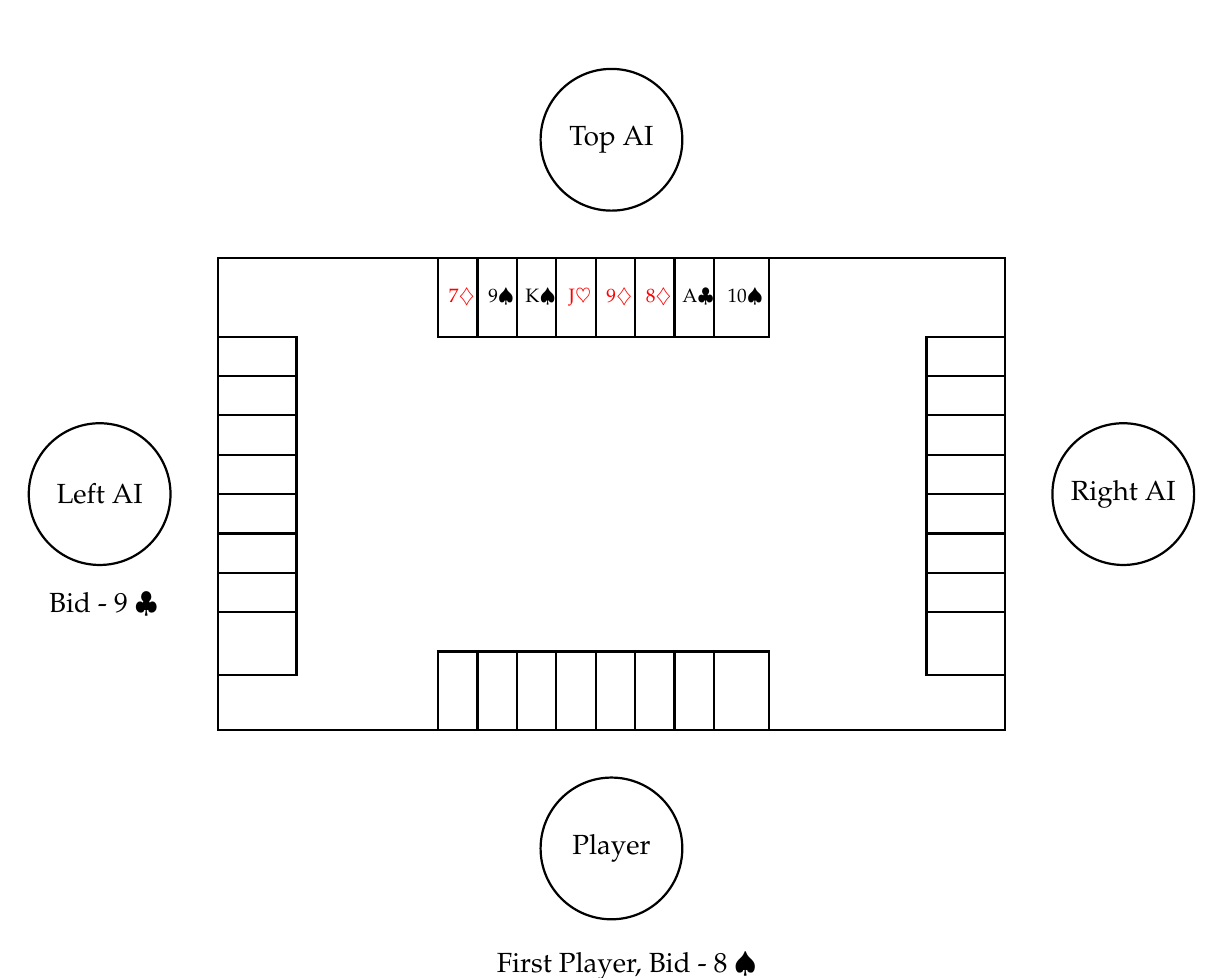
\begin{tikzpicture}

\draw[thick] (0,0) rectangle (10,6);  % Rectangle table dimensions

\foreach \i in {0,1,2,3,4,5,6,7}
    \draw[thick, draw=black, fill=white] (1, 5-\i*0.5) rectangle (0, 5-\i*0.5-0.8);
\foreach \i in {0,1,2,3,4,5,6,7}
    \draw[thick, draw=black, fill=white] (10, 5-\i*0.5) rectangle (9, 5-\i*0.5-0.8);
\foreach \i in {0,1,2,3,4,5,6,7}
    \draw[thick, draw=black, fill=white] (2.8 + \i*0.5, 6) rectangle (3.5 + \i*0.5, 5);
\foreach \i in {0,1,2,3,4,5,6,7}
    \draw[thick, draw=black, fill=white] (2.8 + \i*0.5, 0) rectangle (3.5 + \i*0.5, 1);

\draw[thick] (-1.5, 3) circle(0.9);
% Right side chair
\draw[thick] (11.5, 3) circle(0.9);
% Top side chair
\draw[thick] (5, 7.5) circle(0.9);
% Bottom side chair
\draw[thick] (5, -1.5) circle(0.9);

\node at (-1.5, 3) {Left AI};
\node at (-1.45, 1.6) {Bid - 9 $\clubsuit$};
\node at (11.5, 3) {Right AI};
\node at (5, 7.5) {Top AI};
\node at (5, -1.5) {Player};
\node at (5.2, -3) {First Player, Bid - 8 $\spadesuit$};

\node at (3.1, 5.5) {\scriptsize \textcolor{red}{7$\diamondsuit$}};
\node at (3.6, 5.5) {\scriptsize \textcolor{black}{9$\spadesuit$}};
\node at (4.1, 5.5) {\scriptsize \textcolor{black}{K$\spadesuit$}};
\node at (4.6, 5.5) {\scriptsize \textcolor{red}{J$\heartsuit$}};
\node at (5.1, 5.5) {\scriptsize \textcolor{red}{9$\diamondsuit$}};
\node at (5.6, 5.5) {\scriptsize \textcolor{red}{8$\diamondsuit$}};
\node at (6.1, 5.5) {\scriptsize \textcolor{black}{A$\clubsuit$}};
\node at (6.7, 5.5) {\scriptsize \textcolor{black}{10$\spadesuit$}};

\end{tikzpicture} \pagebreak

If at the start of the game you recalled 8 Spades, and the opponent (Left AI), raised the bid to 9 Clubs,
your partner’s algorithm will look into the hand; say it has these cards (7$\diamondsuit$, 9$\spadesuit$, King$\spadesuit$,
Jack$\heartsuit$, 9$\diamondsuit$, 8$\diamondsuit$, Ace$\clubsuit$, 10$\spadesuit$). The heuristic value for each of the suits would be;

\begin{itemize}
    \item Diamonds:  14 = 0 (8$\diamondsuit$) + 14 (9$\diamondsuit$) + 0 (7$\diamondsuit$),
    \item Spades: 32 = 4 (King$\spadesuit$) + 14 (9$\spadesuit$) + 10 (1$\spadesuit$0) + 1/2 x 8 (Partner’s Bid),
    \item Hearts: 20 (Jack $\heartsuit$),
    \item Clubs: 6.5 = 11 (Ace$\clubsuit$) - 1/2 x 9  (Opponents’ Bid),
    \item No Trumps: 25 = 4 (King$\spadesuit$) + 19 (Ace$\clubsuit$) + 2 (Jack$\heartsuit$)
\end{itemize}

Here it is obvious that the AI
is going to call its partner’s bid (Spades, as it has the highest heuristic value), the question is: How much? There is another logic
imported that would decide if there is a need for the AI to increase the bid by 1, 2 or
more, and the main logic is going to contain the possible additional points from special
combinations (like Tierce giving 2 points), it will also include the bade suit heuristic
value divided 20 (as each 10 heuristic equals to 1 point, and divided with another 2 for emergency)
and rounded and will be added to the point
count, in this case we will have a Tierce (7$\diamondsuit$, 8$\diamondsuit$, 9$\diamondsuit$) and heuristic difference of 32/20
= 1.6, rounded to 2. The point count would include adding 4 points to the partner’s bid,
hence the algorithm will return 12 Spades. There are going to be extra conditions for
the actions Coinchee, Cabot, etc.)


\subsection{Minimax Algorithm for the Playing part}
\hspace{\parindent} Up to the Second phase of the game, which is the playing process.
In this case, we will use
the Stochastic Minimax Algorithm, which will work for each trick (each player making one
move after which it is calculated which side gets the cards). At the beginning of the
game, there will be a set trump, which will prioritize the moves of the players,
especially if their bid won. If your bid did not win, and the play starts with you,
the minimax algorithm will prioritize using high value non-trump cards, however, the
algorithm should check, if the opponents will either have a higher value card from the
same suit, or no cards of the corresponding suit. As an example, Let’s imagine that the
play starts with the AI, the bid belongs to opponents, and it is set to be 11$\spadesuit$.
The bot has 1 trump card (Q$\spadesuit$), 3$\clubsuit$, 2$\diamondsuit$, and 10$\heartsuit$. The highest
non-trump card is 10$\heartsuit$. The Minimax algorithm, will check all the branches with
possible combinations of 8 cards for the opponent, and return possibilities for cases
when the bot team wins, or when the opponents win. In this case, it would be 2/3 chance
for the opponents to have the Ace$\heartsuit$, 1/3 chance for the partner to have Ace$\heartsuit$. We add
to this the probability that one of the opponents does not have any Hearts hence they
will use the trump. If we approximate, we will calculate the chances of not having any
of the remaining 6 hearts out of 24 (p=0.25) and calculate the probability using Binomial
Distribution on 8 cases with 0 successes, returning 0.1 for each player (chance of not
having a Hearts card). For at least one player to not have any hearts card, we will get
19% chance for at least one of the opponents not having any Hearts. As a result we would
get the union of the probabilities and get the 86% chance of losing the H10 by playing it.
Hence the Stochastic Minimax will play
the card with 86% chance. Instead of using Binomial Distribution, the algorithm will
check the possible outcomes of the play, and calculate the proportion, when the H10 is
lost to opponents, and hence get the probability of success. This process would be done
for each prioritized card to play, until the best option is picked (Highest success rate).
If the bot is prone to lose the card nonetheless, then it is chosen to be the least value
having card on the hand.


% Appendices, remove if unused

% Bibliography
\newpage
\thispagestyle{SectionFirstPage} % Hide headers on the first page of the section
\lhead{References}
\rhead{}
\renewcommand\refname{References}
\printbibliography
\end{document}
